\chapter{Results}

With the extensions and modifications I developed, it became possible to consume SOAP web services using WS-Security authentication methods with Python clients. Since I found no evidence, that it was possible before, I don't compare the solution to others in the Python ecosystem, but with the implementation I used as a reference, Apache CXF.

\section{Timing measurement}

\subsection{Methodology}

I extended the \emph{Arena} testbed (see section \ref{arena}) with the option of measurement, which had a number of advantages. It ensured, that all runs were correct, and it already had the knowledge to arrange a ``rendezvous'' between services and consumers. The items added to the structure seen on Figure \ref{fig:clsdArena} were configurations and repeat values.

\begin{description}
 \item[Configurations] These define environment values, which are available to both the service and the consumer, thus are perfect to let them know about the parameters of the service. I defined the following suites to provide a way to get useful measurements.
 \begin{description}
  \item[No security] is without any form of authentication
  \item[Plain UsernameToken] uses UsernameToken with a plaintext password
  \item[Digest UsernameToken] uses UsernameToken with a digested password
  \item[Signed message] uses digital signature without a timestamp
  \item[Signed message w/ TS] uses digital signature with a timestamp
 \end{description}
 \item[Repeat values] The repeat values are important for the measurements to get a clear picture about the fixed and variable costs of the SOAP processing. I chose \textbf{1, 10 and 100}, as they provide reasonably fine enough resolution, while keeping runtime low.
\end{description}

\noindent
I put code into both consumers (CXF and SUDS) that measured two values.
\begin{description}
 \item[Proxy initialization] measures the time needed to create a proxy instance that can be used to invoke service methods. The measurement is started as the first statement after the entry point, and is stopped right after an instance of the service proxy is available in a local variable.
 \item[Invocation round-trip time] measures the time needed to invoke a service method one or more times. The measurement is started as the one for proxy initialization stops, and stops right after the last call has ended.
\end{description}

\noindent
In measurement mode, the \emph{Arena} testbed creates two files -- named using the timestamp at program startup -- a log file and a CSV table. The log file is written only by the \emph{Arena} measurement module, and currently contains one timestamped line for every test started. The CSV table on the other hand receives only the header from \emph{Arena}, its contents are produced by the consumers. They get the name of the CSV file and a prefix that contains the parameters of the current test through environment values, and using this, the two time measurements can be appended to the table. After the tests have run, the CSV table contains all the necessary data for timing analysis readable by any spreadsheet software.

\subsection{Environment}

For the sake of simplicity, I kept the setup used by \emph{Arena}, so the service and the consumer under test ran on the same host, and the loopback interface was used for network interconnection. The full network traffic of the measurement was captured using Wireshark and saved for later analysis -- this way, its overhead affected all test runs equally. This made it also easy to check later, that no other traffic went through the loopback interface used, thus providing equal circumstances. The exact components along with their version numbers and relations can be seen on Figure \ref{fig:measurenv} and Table \ref{tab:measurenv}. Note, that the composite relationship between the \emph{Arena} and the other processes describes the one between a process and a subprocess, while the cloud and the lightning symbols represent the network interconnectivity through the loopback interface, which is ``bootstrapped'' using information passed through environment values.

\begin{figure}[htbp]
 \centering
 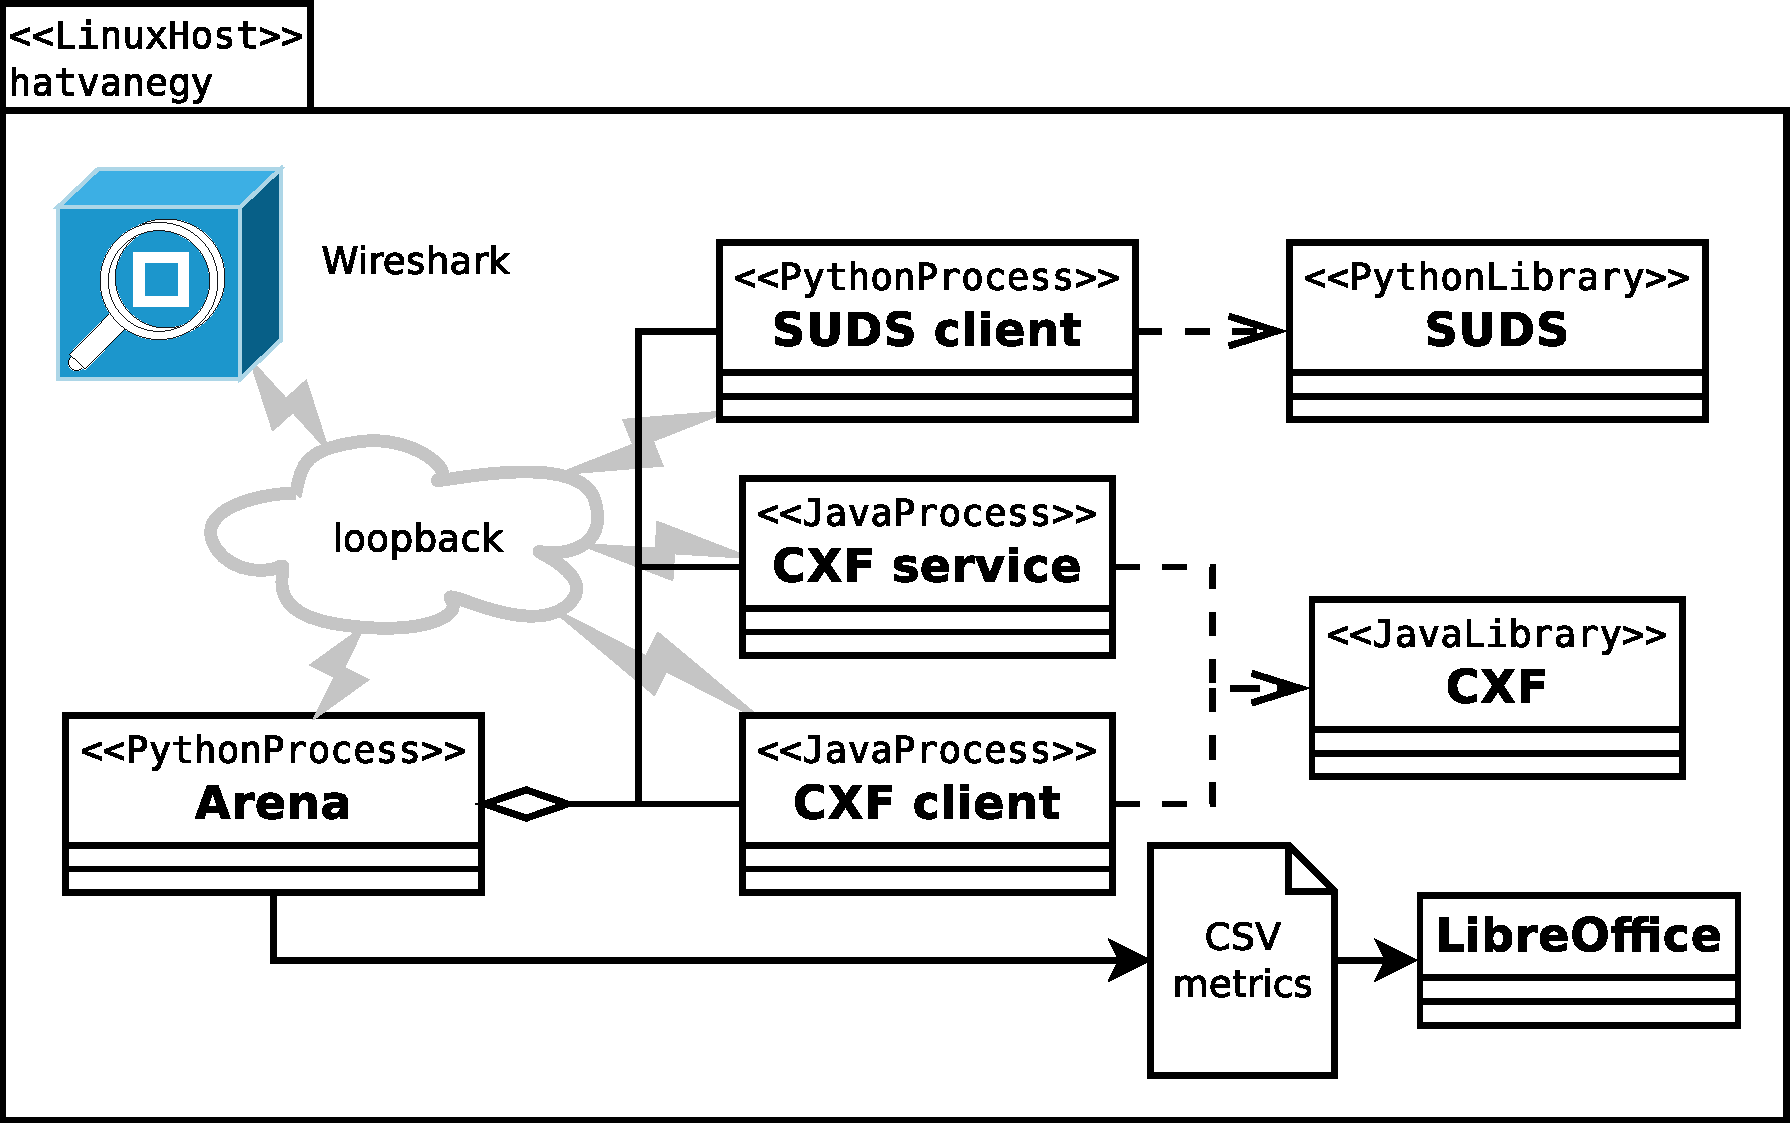
\includegraphics[width=0.9\textwidth]{images/measurenv.pdf}
 \caption{Structural diagram of the measurement environment}
 \label{fig:measurenv}
\end{figure}

\begin{table}[htbp]
 \centering
 \toprule
 \begin{minipage}[t]{0.55\linewidth}
  \centering
  \begin{tabular}{rl}
  \textbf{CPU} & Intel Core 2 Duo T7300 @ 2 GHz \\
  \textbf{RAM} & 4 GB \\
  \textbf{OS} & Debian GNU/Linux 7.0 ``Wheezy'' \\
  \textbf{Kernel} & Linux 3.1.0 / i686 \\
  \textbf{JRE} & Oracle Java SE 1.6.0\_26 \\
  \end{tabular}
 \end{minipage}
 \begin{minipage}[t]{0.3\linewidth}
  \centering
  \begin{tabular}{rl}
  \textbf{CXF} & 2.5.0 \\
  \textbf{Python} & 2.7.2 \\
  \textbf{SUDS} & 0.4.1 \\
  \textbf{Wireshark} & 1.7.0 \\
  \textbf{LibreOffice} & 3.4.4
  \end{tabular}
 \end{minipage}
 \bottomrule
 \caption{Attributes and version numbers of the measurement environment}
 \label{tab:measurenv}
\end{table}

\section{Timing analysis}

\subsection{Network traffic}
\label{traffic}

\begin{table}[htbp]
 \begin{center}
  \input{stat_packet}
  \caption{Network traffic generated by CXF and SUDS invocation}
  \label{tab:stat_packet}
 \end{center}
\end{table}

\noindent
The amount of network traffic generated by an invocation becomes less of an issue as network throughtput and latency continuously gets improved, although having perfect interconnections in every part of the system is far from reality. I used the TCP conversations module of the Wireshark analysis module, and put the results into Table \ref{tab:stat_packet}, which highlights a serious issue. Even in case of a single request, SUDS generates 33\% more packets as CXF, and at 100 requests, the difference becomes 250\%. The cause is simple; the current implementation of SUDS uses \emph{urllib2}, part of the Python base library, as I wrote in section \ref{sudsInvocation}. This solution opens a new TCP connection for each HTTP request by default, which causes overhead, especially a problem in case of HTTPS, which requires a TLS handshake in addition to the TCP one. Since this disadvantage of SUDS is unrelated to its architecture, I propose a soluton in Section \ref{keepalive}.

\subsection{Proxy initialization}

\begin{table}[htbp]
 \begin{center}
  \input{stat_init}
  \caption{Time needed for CXF and SUDS proxy initialization}
  \label{tab:stat_init}
 \end{center}
\end{table}

\noindent
The first thing that catches the eye on Table \ref{tab:stat_init} is that SUDS instantiates the proxy in less then half the time CXF needs to perform the same, regardless the configuration. It's also interesting to see, that according to these timings, SUDS needs an additional \mbox{210 ms} on average in case of digital signatures, whereas CXF takes roughly the same time in every case. The most logical explanation to me is that in the SUDS client, library import is done on demand, so this extra time is what it takes to load the LXML, libxml2 and XMLSec libraries, latter two requiring native components.

\subsection{Invocation round-trip time}

\begin{table}[htbp]
 \begin{center}
  \input{stat_invoke}
  \caption{Time needed for CXF and SUDS invocation}
  \label{tab:stat_invoke}
 \end{center}
\end{table}

\noindent
Per-invocation round-trip times are more interesting to architects, especially when designing consumers with more than one call to the service, and Table \ref{tab:stat_invoke} shows interesting differences between the two solutions. In case of a single invocation, CXF takes double the time SUDS needs, but this gain decreases with the number of requests increasing, and at 100 calls without digital signatures, CXF performs 1--5\% better. On the other hand, even 100 digitally signed messages are handled in almost 10\% less time by SUDS, probably caused by the elevated use of native components.

\section{Architectural differences}

\subsection{Runtime environment}

Apache CXF runs on Java VMs, most notably the one Oracle produces. This limits its usage to -- both hardware and software -- platforms it supports, and at the same time, it makes CXF a good choice in case of an application server (for example Glassfish) that only supports Java code. In a similar way, SUDS requires a Python runtime, although SUDS itself depends on such libraries, that its code can be compiled to Java or .NET bytecode, and it can run on Nokia S60 smartphones. A constraint comes with the \emph{SudsSigner} component I developed, which uses multiple native components, as it limits its use to the CPython environment.

Because of this, they're not that much competitors, since in case of a pre-existing system, compatibility with the selected runtime will decide. But on the other hand, in case of newly built systems, choosing Java vs. Python for a system that needs to consume advanced SOAP web services will be a decision with ``real'' alternatives.

\subsection{Use of native components}

For reasons of performance and reuse, I chose to depend on native components while implementing the \emph{SudsSigner} component for SUDS. The timings clearly show, that using native code improves performance; my proof-of-concept quality code beat the one of many talented CXF developers. Based on this, one may draw the conclusion, that the usage of native components is a clear advantage -- but it's far from the truth. The disadvantage is, that in case of managed components, all the code runs protected by additional safeguards, and officially, the worst thing that can happen is an exception being thrown, whereas with native components, the whole OS process can crash without prior notice.

The fact that it's not a theoretical problem is proven by events that happened to me while working on XML digital signatures with both sec-wall and SUDS. As I said in section \ref{lxml}, LXML is preferred as it encapsulates low level issues with exceptions, so when I was busy developing with direct libxml2 and XMLSec, I got surprised by the fact, that a single mistake in my code can lead to for instance null pointer dereferences, which in turn cause immediate crash (segmentation fault). Long story short: native components might give performance gains, but it's important to check the price tag.

\chapter{Summary}

\section{Results summary}

As a result of my work, SUDS now has correct UsernameToken and digital signature implementation, which is a unique capability in the Python SOA world. I created an extensible testbed called \emph{Arena}, and continuously tested the interoperability of my solution with an Apache CXF service during the development. When I considered the proof-of-concept code ready, I added measurement instrumentation to the testbed, and analyzed the timings and the network traffic of both the SUDS and the CXF consumer. As it turned out, my solution performed reasonably well, although I found plenty room for improvement.

\section{Future development opportunities}

Since most of the solutions in the Python ecosystem are free software in both senses\footnote{free as in free beer vs. free as in free speech}, software is continuously improved by its community following the needs of their members. For instance, during my thesis, I also created and published a proof-of-concept code to handle messages with attacments, and an interested user developed it further since to the point of real world usability. The following three goals are those, I think can and should be done in order to further improve Python SOA solutions.

\subsection{Short-term: taking advantage of HTTP keep-alive}
\label{keepalive}

The HTTP implementation used by SUDS generates network overhead, as I shown in section \ref{traffic}. Several ways exist to solve this issue -- as explained in \cite{so-1037406} -- some require replacing \emph{urllib2} with a whole new library, others just require extending it with plugins (so-called \emph{openers}) -- two things are for sure; it requires more than a simple method call, and the solution must be carefully tested for compatibility with different versions of its dependencies. Still, it only affects a relatively isolated part of the codebase, and would improve performance regardless of any optional (security) features.

\subsection{Mid-term: implementing XML encryption}

As I mentioned in section \ref{xmlenc}, as of 2011, the XML encryption standard is considered broken, so implementing it would do little or no good -- in my opinion, false belief in security is worse than no security at all. But as the future goes, XMLSec supports XML encryption, so in case the library is updated against the new design, it'd be fairly straightforward to make use of it in SUDS and sec-wall. I consider it a mid-term goal, since in this case (in contrast with digital signature), it makes more sense to use encryption on the response too, so the solution should be usable in both scenarios. By looking at Figure \ref{fig:sudsMessage}, it's clear, that the \emph{received} hook could be used to construct a message plugin the same way I did implementing the \emph{SudsSigner}.

\subsection{Long-term: wider cryptographic backend support}

The current \emph{SudsSigner} implementation supports only DSA and RSA digital signatures, and while these are quite common because of the ubiquity of PKI implemented with X.509 certificates, the WS\hyp{}Security standard -- or more specifically, the XML Signature W3C Recommendation -- contains guidelines for OpenPGP, too. As the main developer, Aleksey Sanin wrote in \cite{aleksey-pgp-mail}, XMLSec could have had PGP support, but he had problems regardning the availability and licensing of the necessary library. Two years later, John Belmonte wrote in \cite{belmonte-pgp-mail}, that he took part in a project that implemented PGP XML digital signatures in Python, although it seems by his words, that the product is closed source. That said, it doesn't seem impossible to add PGP support into XMLSec, using an appropriate library -- and GPGME \cite{gpgme-homepage} seems like the best candidate.
